\documentclass[border=10pt]{standalone}
\usepackage[T1]{fontenc}
\usepackage{tikz}
\usepackage[svgnames]{xcolor}
\usetikzlibrary{shapes.geometric, arrows.meta, positioning, calc, fit}

\colorlet{OrangeFill}{LightSalmon}
\colorlet{OrangeLine}{DarkSalmon!30!Chocolate}
\colorlet{GreenFill}{MediumAquamarine}
\colorlet{GreenLine}{MediumAquamarine!30!Teal}
\colorlet{PurpleFill}{MediumPurple}
\colorlet{PurpleLine}{MediumPurple!30!SlateBlue}
\colorlet{PinkFill}{Thistle}
\colorlet{PinkLine}{Thistle!30!Plum}
\colorlet{BlueFill}{LightSkyBlue}
\colorlet{BlueLine}{SteelBlue}
\colorlet{GrayFill}{LightGray!60!OldLace}
\colorlet{GrayLine}{RosyBrown!50!Silver}

\begin{document}
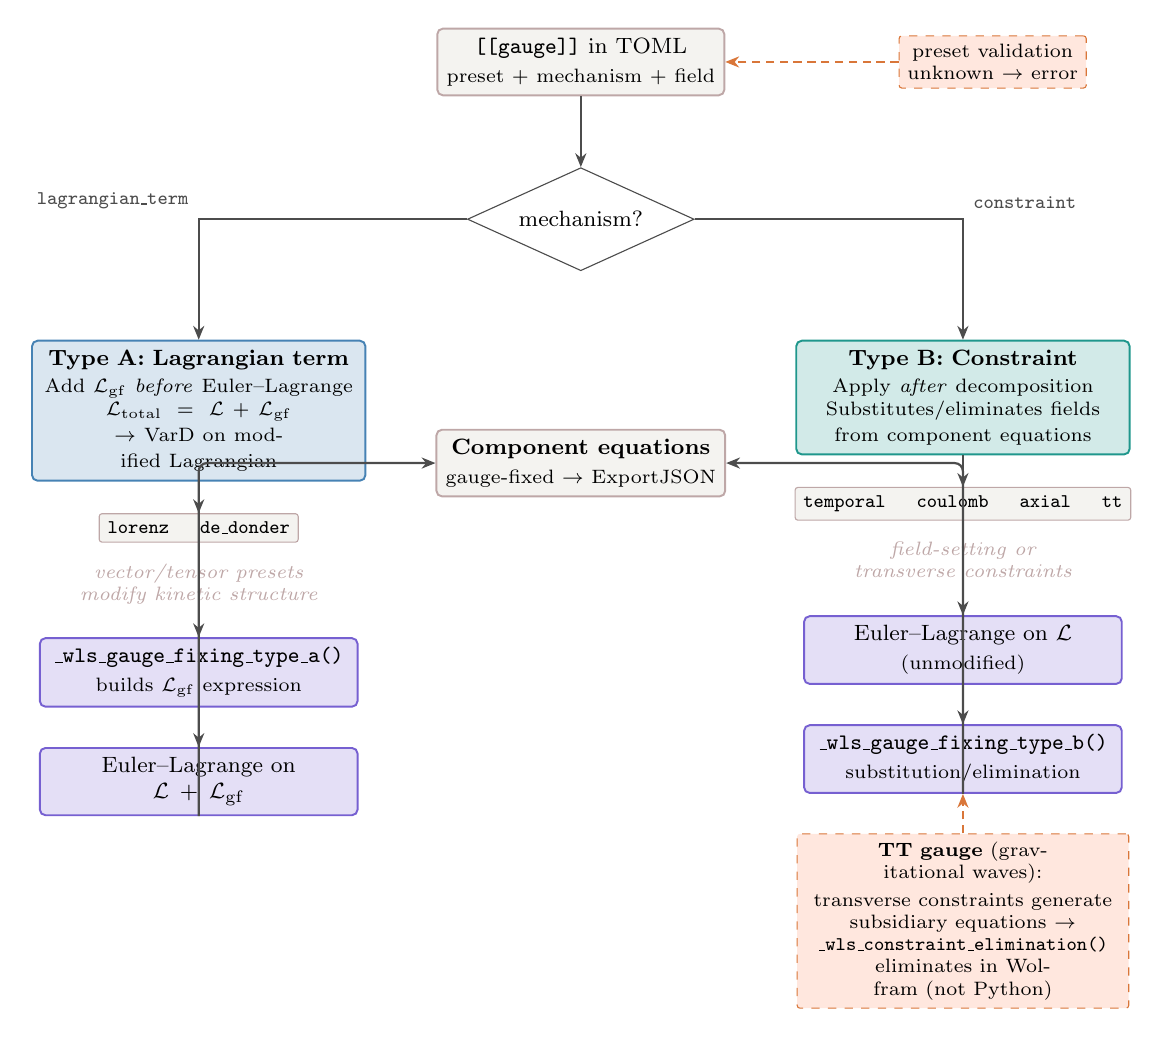
\begin{tikzpicture}[
    stage/.style={
        rectangle, rounded corners=2pt, minimum width=3.0cm,
        minimum height=0.7cm, draw=#1, line width=0.7pt,
        fill=#1!20, font=\footnotesize, align=center,
        text opacity=1, text=black
    },
    stage/.default={black!70},
    decision/.style={
        diamond, aspect=2.2, minimum width=1.6cm,
        draw=black!70, fill=white, font=\footnotesize,
        align=center, inner sep=2pt, text width=2.0cm
    },
    preset/.style={
        rectangle, rounded corners=1pt, draw=GrayLine,
        fill=GrayFill, fill opacity=0.4, font=\scriptsize\ttfamily,
        align=center, text opacity=1, inner sep=3pt
    },
    check/.style={
        rectangle, rounded corners=1pt, draw=OrangeLine, dashed,
        fill=OrangeFill, fill opacity=0.25, font=\scriptsize,
        align=center, text opacity=1, inner sep=3pt
    },
    annot/.style={font=\scriptsize\itshape, text=GrayLine, align=center},
    arr/.style={-{Stealth[length=5pt, width=4pt]}, thick, black!70},
    yeslbl/.style={font=\scriptsize\bfseries, text=black!70},
    node distance=0.7cm and 2.4cm
]

% ===================================================================
% ENTRY
% ===================================================================
\node[stage=GrayLine, fill=GrayFill, fill opacity=0.4] (toml)
    {\textbf{\texttt{[[gauge]]}} in TOML\\[1pt]
     \scriptsize preset + mechanism + field};

\node[check, right=2.2cm of toml] (validate)
    {preset validation\\unknown $\to$ error};
\draw[arr, densely dashed, OrangeLine] (validate) -- (toml);

% ===================================================================
% DECISION: mechanism
% ===================================================================
\node[decision, below=0.9cm of toml] (dmech)
    {mechanism?};

\draw[arr] (toml) -- (dmech);

% ===================================================================
% TYPE A: Lagrangian term (left branch)
% ===================================================================
\node[stage=BlueLine, below left=1.2cm and 2.0cm of dmech,
      text width=4.0cm] (typeA) {%
    \textbf{Type A: Lagrangian term}\\[2pt]
    \scriptsize Add $\mathcal{L}_{\mathrm{gf}}$ \emph{before} Euler--Lagrange\\
    \scriptsize $\mathcal{L}_{\mathrm{total}} = \mathcal{L} + \mathcal{L}_{\mathrm{gf}}$\\
    \scriptsize $\to$ VarD on modified Lagrangian};

\node[preset, below=0.4cm of typeA] (presetsA)
    {lorenz \quad de\_donder};
\node[annot, below=0.15cm of presetsA]
    {vector/tensor presets\\modify kinetic structure};

\draw[arr] (dmech.west) -| node[yeslbl, above left]
    {\texttt{lagrangian\_term}} (typeA.north);

% Type A stages
\node[stage=PurpleLine, below=1.2cm of presetsA, text width=3.8cm] (buildA)
    {\texttt{\_wls\_gauge\_fixing\_type\_a()}\\[1pt]
     \scriptsize builds $\mathcal{L}_{\mathrm{gf}}$ expression};

\node[stage=PurpleLine, below=0.5cm of buildA, text width=3.8cm] (elA)
    {Euler--Lagrange on\\$\mathcal{L} + \mathcal{L}_{\mathrm{gf}}$};

\draw[arr] (typeA) -- (presetsA);
\draw[arr] (presetsA) -- (buildA);
\draw[arr] (buildA) -- (elA);

% ===================================================================
% TYPE B: Constraint (right branch)
% ===================================================================
\node[stage=GreenLine, below right=1.2cm and 2.0cm of dmech,
      text width=4.0cm] (typeB) {%
    \textbf{Type B: Constraint}\\[2pt]
    \scriptsize Apply \emph{after} decomposition\\
    \scriptsize Substitutes/eliminates fields\\
    \scriptsize from component equations};

\node[preset, below=0.4cm of typeB] (presetsB)
    {temporal \quad coulomb \quad axial \quad tt};
\node[annot, below=0.15cm of presetsB]
    {field-setting or\\transverse constraints};

\draw[arr] (dmech.east) -| node[yeslbl, above right]
    {\texttt{constraint}} (typeB.north);

% Type B stages
\node[stage=PurpleLine, below=1.2cm of presetsB, text width=3.8cm] (elB)
    {Euler--Lagrange on $\mathcal{L}$\\[1pt]
     \scriptsize (unmodified)};

\node[stage=PurpleLine, below=0.5cm of elB, text width=3.8cm] (applyB)
    {\texttt{\_wls\_gauge\_fixing\_type\_b()}\\[1pt]
     \scriptsize substitution/elimination};

\draw[arr] (typeB) -- (presetsB);
\draw[arr] (presetsB) -- (elB);
\draw[arr] (elB) -- (applyB);

% ===================================================================
% TT GAUGE SPECIAL CASE
% ===================================================================
\node[check, below=0.5cm of applyB, text width=4.0cm] (ttcheck) {%
    \textbf{TT gauge} (gravitational waves):\\[2pt]
    transverse constraints generate\\
    subsidiary equations $\to$\\
    \texttt{\_wls\_constraint\_elimination()}\\
    eliminates in Wolfram (not Python)};
\draw[arr, densely dashed, OrangeLine] (ttcheck) -- (applyB);

% ===================================================================
% CONVERGENCE: both paths → JSON
% ===================================================================
\node[stage=GrayLine, fill=GrayFill, fill opacity=0.4,
      below=2.0cm of dmech] (json)
    {\textbf{Component equations}\\[1pt]
     \scriptsize gauge-fixed $\to$ ExportJSON};

\draw[arr, rounded corners=3pt] (elA.south) |- (json.west);
\draw[arr, rounded corners=3pt] (applyB.south) |- (json.east);

\end{tikzpicture}
\end{document}
